\documentclass[12pt]{texMemo}  
\usepackage[english]{babel}
\usepackage{graphicx, blindtext, setspace, amsmath, amssymb, natbib}
\memoto{Adrienne Davis, Vice Provost}
\memofrom{Jacob M. Montgomery}
\memosubject{The Status of Women in the Political Methodology Subfield}
\memodate{\today}

\usepackage{booktabs}
\begin{document}

\newcommand{\stcomp}[1]{{#1}^\complement}

{\begin{center}
\Large\bf
M\textsc{emorandum}
\end{center}}



\maketitle
\singlespacing

\section*{Introduction}

Political methodology is a subfield of political science focused on research methodology and design, data collection,  measurement, statistics, and empirical modeling in Political Science. Political methods as a distinct subfield did not exist until the mid 1970s with the first official conference of the Society for Political Methodology (SPM) occurring in 1983.  Political methodology has expanded significantly as quantitative approaches to research have increasingly dominated the discipline.  

However, even from its earliest days the methods subfield has struggled to diversify.\footnote{Methods has also struggled extremely with including persons of color -- especially under represented minorities.  However, the focus of this memo is on the status of women.}  Accounts of the early meetings of the SPM indicate they were almost exclusively male. And, while progress has been made, the field still lags far behind the broader discipline. Like other STEM fields, political methodology struggles to recruit women graduate students and suffers from a ``leaky pipeline'' all the way up the academic ladder.  The net consequence is that political methods is \textit{the least diverse subfield in all of political science}. 


\section*{Women in political methodology}

\subsubsection*{Our search pool}

Members of the search committee spent considerable time and effort recruiting applicants with special attention paid to identifying women and under-represented minorities.  Nonetheless, only 12 out of the 73 files we received (16.4\%) were from women.  To put this in contrast, the candidate pools for our searches last year in American politics and comparative politics were  28\% women and  24\% respectively. 


The poor numbers in our pool are not an abberation.  Rather, as I show below, they are a symptom of a larger (and very serious) gender representation problem in the methods field.  


\subsubsection*{APSA organized section}

The American Political Science Association (APSA) reports that 36.7\% of its members are women.  However, when we break this down by section, it is clear that women are very unevenly distributed across subfields.  Figure 1 shows the percent of women in 43 of APSA's organized sections.\footnote{The Women and Politics Research section (91.6\% women) is excluded.} 
\begin{figure}[htbp]
\caption{Percent of women for APSA organized sections}
\vspace{-.7in}
\begin{center}
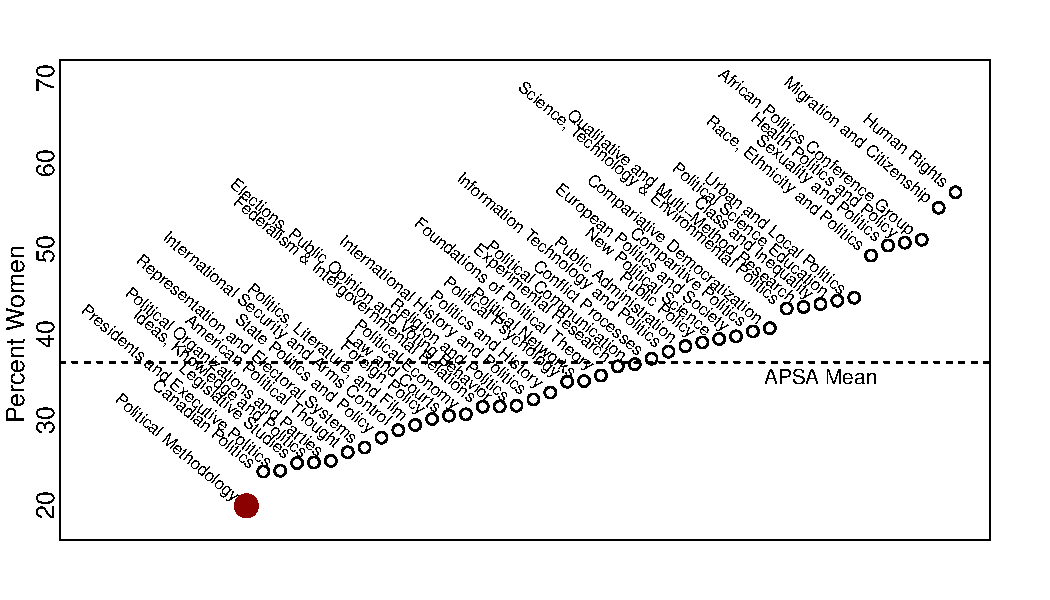
\includegraphics{sections}
\end{center}

\vspace{-1cm}
\footnotesize Data comes from American Political Science Association.  The Women and Politics Research section (91.6\% women) is excluded from this plot to make it visually clearer. The dashed horizontal line shows the overall percent of women in APSA. 
\end{figure}
From this data it is clear that while many subfields (e.g., legislative studies, American political thought, etc.) include fewer women than the APSA average, political methodology is a clear outlier.  In all, only 19.2\% of the membership of this section are women.

\subsubsection*{APSA conference participation}

Another way to examine the representation of women in the field is to look at conference participation.  Therefore, I collected the names of all participants at APSA's annual meeting held in San Francisco in August 2017 who were on a panel sponsored by the political methodology division.  All participants were coded by gender.  The results, shown in Figure 2, indicate that only 19\% of methods panelists at our discipline's most prestigious conference were women.
\begin{figure}[htbp]
\caption{Gender breakdown of APSA 2017 Methods Panels}
\begin{center}
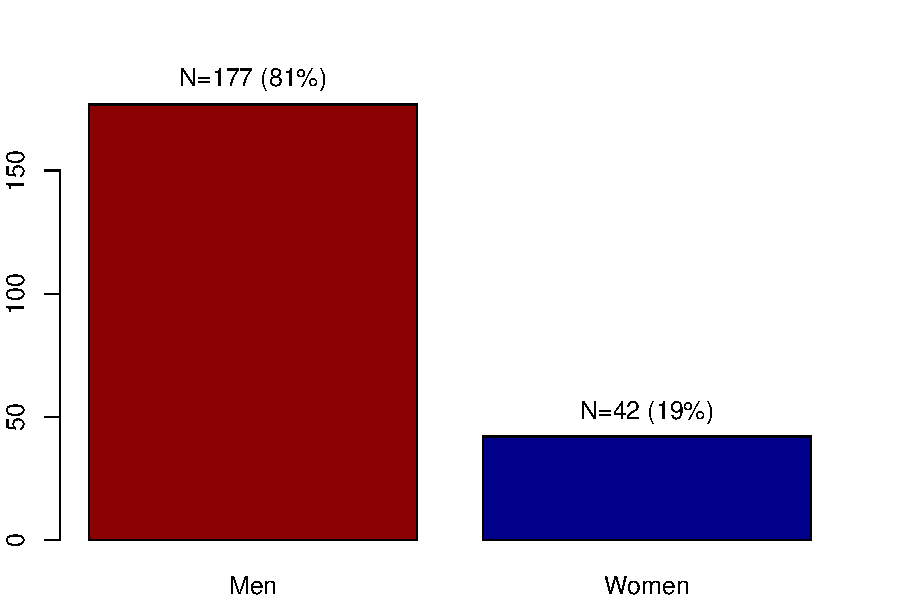
\includegraphics[scale=.6]{apsaGender}
\end{center}


\footnotesize Data collected from the 2017 APSA online program.
\end{figure}

\subsubsection*{SPM summer meeting}

From its origins, the annual summer meeting of the SPM has played a crucial role in defining the political methods field and its membership.  For this reason, the \textit{National Science Foundation} has provided extensive support to SPM to include more women and minorities at the annual conference.  These funds are mostly used to cover the costs of graduate students to attend.

At the 2017 SPM meeting held in Madison Wisconsin, 57 out of 211 participants were women (27\%).  While an improvement over APSA, these numbers are actually somewhat deceptive since they obscure other serious gender representation issues.   
\begin{figure}[htbp]
\caption{Gender breakdown of 2017 SPM conference by status/participation }
\begin{center}
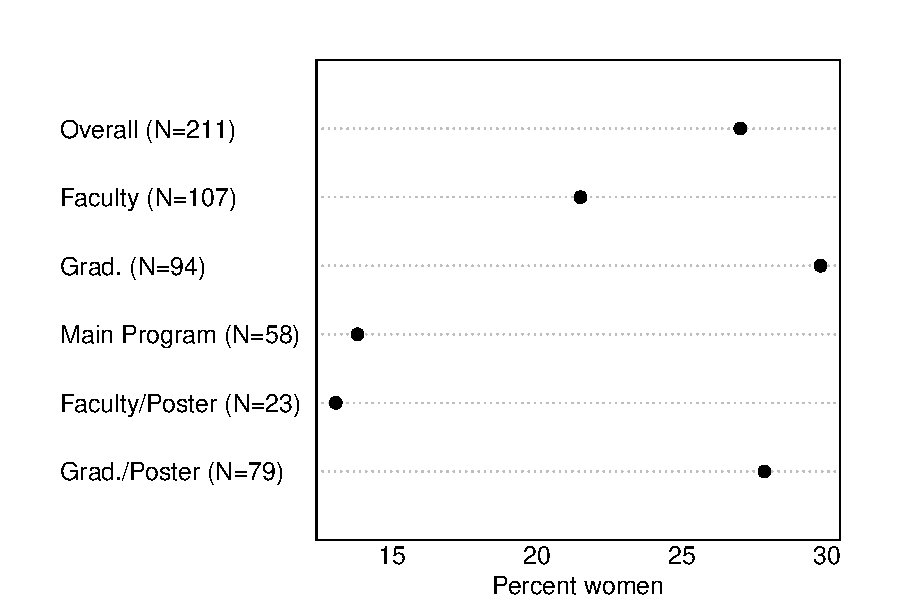
\includegraphics[scale=.8]{polmeth}
\end{center}


\footnotesize Data provided by the Society for Political Methodology and coded from the from the 2017 Polmeth program.
\end{figure}
First, while 27\% of conference participants were women only 21.4\% of participants on tenure track jobs were women.  That is, the somewhat better numbers for women relative to APSA only holds among graduate students (29.8\% women).  

Second, gender representation is actually worse if we focus only on individuals who actually appeared on the conference program.  Only 13.8\% of individuals who presented or discussed research in one of the panels were women.  Only 13\% of tenure-track faculty who presented posters were women.  Graduate students are only allowed to present posters at this conference, and the numbers are somewhat better (27.8\%).  But even here, fewer women presented research on posters than we would expect from the overall proportion of women graduate students (29.8\%).

\newpage

\subsubsection*{Tenured women methodologists}

As stark as the numbers above are, I will close by pointing out that they are even worse at more senior levels. I am aware of only 13 tenured women in the political methodology field (using a very broad definition) and only eight full professors.\footnote{Janet Box-Steffensmeir (Ohio State), Suzanna Linn (Penn State), Wendy Tam Cho (Illinois), Lonna Atkinson (New Mexico), Betsy Sinclair (WUSTL), Rocio Titiunik (Michigan), Vera Troeger (Warwick), Xun Pang (Tsinghua University), Sunshine Hillygus (Duke), Sarah Mitchel (Iowa), Jennifer Victor (George Mason), Amber Boydston (UC-Davis), Becky Morton (NYU) } At top-25 departments (as ranked by the US News and World Report) there are only seven tenured faculty and only four full professors. 




\end{document}